\chapter{Metodika}


%V této části buďte velmi precizní. Vše musíte popsat tak důkladně, aby kdokoliv mohl vaše pokusy či
%pozorování zopakovat. Nezapomeňte uvést velikost vzorků, věk a pohlaví zvířat, denní a roční dobu,
%podmínky chovu nebo popis lokalit (třeba včetně mapky), specifické přístrojové vybavení
%(pokud je to důležité, např.~pro srovnání výsledků s publikovanými údaji, uveďte i přesný typ
%přístroje) a jiné podrobnosti. Také může být dobré zmínit, jak jste zabránili vlivu pakovaného testování stejných
%individuí a proč se domníváte, že je počet jedinců dostatečný k zodpovězení vašich otázek. Více než
%vhodné je zmínit a zdůvodnit použité statistické metody a počítačové programy. Používáte-li zkratky, uveďte
%jejich seznam.
%Materiál a metodika bývají pro větší srozumitelnost často členěny na menší podkapitoly: materiál,
%experimentální design, analýza dat atd. Systém více podkapitol třeba jen o třech řádcích bývá přehlednější
%než souvislý odstavec na dvě strany. (A to samozřejmě neplatí jen pro metodiku.)
%Čtení DP usnadní, pokud je členění na podkapitoly obdobné v kapitolách Materiál a metodika,
%Výsledky a případně i Diskuse.
%Při vší pečlivosti se však snažte být poměrně struční. Materiál a metodika by neměly tvořit většinu DP.

XXX neco trosku obecnejsiho?

\section{Simulace}

Použil jsem stochastický model postavený na individuích. Individua jsou jedinci jednoho druhu s oddělenými pohlavími a
žijí v nestrukturovaném prostředí. Fenotyp jedinců i optimum prostředí jsou čtyřrozměrnými vektory.
Optimum prostředí $E(t)$ není stálé, ale může se měnit v čase.
Euklidovská vzdálenost fenotypu jedince od aktuálního optima prostředí určuje jeho fitness.

Optimum prostředí je po dobu 2048 kroků simulace konstantní a následně dojde k jeho skokové změně o
$\Delta{}E$. Po této změně opět zůstane optimum neměnné.

Počáteční velikost populace je jedním z parametrů simulace. V~dalších krocích je následně velikost populace udržována
mechanismem turbidostatu.
Navíc je každý jedinec limitován maximální délkou života -- po 64 (XXX) krocích umírá.
Jedinci jsou sexuálně dospělí ihned v následujícím kroku simulace a věk neovliňuje jejich fenotyp.



XXX picture: Big picture



V každém kroku jsou z populace náhodně vybrány páry opačného pohlaví a osmina z nich se může rozmnožit.
Kolik vyvedou potomků, je určeno průměrnou fitness páru. Způsob, jak je jsou určeny počty potomků, jejich geny a
jak následně geny určují jejich fenotyp, je popsán později.
Při každém kroku simulace také velmi malou část jedinců postihne mutace jednoho nebo více genů.

\section{Jedinec a jeho geny}

Geny každého jedince jsou uloženy v dvou homologních chromosomech. Každý z těchto chromosomů má XXX lokusů.
Na každém z lokusů je alela, která má vliv na fenotyp jedince. Alela je určena svým příspěvkem k fenotypu (čtyřrozměrný
vektor, typicky s jednou nenulovou hodnotou) a svým příspěvkem k fenotypu, pokud se vyskytuje na obou protilehlých
lokusech (opět čtyřrozměrný vektor). Druhý příspěvek k fenotypu se tedy projevuje jako dominance alely.

Na počátku simulace jsou vygenerováni náhodní jedinci. Jejich alely jsou generovány náhodně - příspěvek k fenotypu
má jednu nenulovou složku pro náhoně zvolenou dimenzi. Velikost této složky je vybrána z normálního rozdělení. Vliv na
fenotyp v případě dominance závisí na parametrech simulace. S určenou pravěpodobností je to opačný vektor k běžnému
vlivu na fenotyp, jinak je to nulový vektor.

\subsection{Mutace}

Jedinou možnou mutací je změna alely za jinou - nejsou tedy simulovany rozsahlejsi mutace, ktere maji vetsi vliv na
strukturu DNA.

Nad každým lokusem v obou chromosomech určeno s pravděpodobností XXX, zda u něj dojde ke změně.
V případě, že ano, tak je na lokus dána nová náhodná. Nová alela vybírána obdobným mechanismem, jako jsou
generovny počáteční alely.

\begin{figure}
  \centering

  \begin{tikzpicture}

    \begin{scope}
      \DNASequence[Mutated]{$\blacktriangleright$/white!30,$\clubsuit$/red!30,$\#$/white!30,$\triangleleft$/white!30,$\circ$/white!30,$\flat$/white!30}
    \end{scope}

    \begin{scope}[yshift=1cm]
      \DNASequence{$\triangleright$/white!20,$\clubsuit$/white!30,$\bot$/white!20,$\triangleleft$/white!30,$\bullet$/white!30,$\sharp$/white!30}
    \end{scope}


    \begin{scope}[xshift=9cm]
      \DNASequence[Done]{$\blacktriangleright$/white!30,$\diamondsuit$/red!30,$\#$/white!30,$\triangleleft$/white!30,$\circ$/white!30,$\flat$/white!30}
    \end{scope}

    \begin{scope}[xshift=9cm,yshift=1cm]
      \DNASequence{$\triangleright$/white!20,$\clubsuit$/white!30,$\bot$/white!20,$\triangleleft$/white!30,$\bullet$/white!30,$\sharp$/white!30}
    \end{scope}

    \ConnectNodes[out=-90, in=-30]
        {Done-1.south}
        {Mutated-1.south};

  \end{tikzpicture}

  \caption{Mutace}
\end{figure}

\subsection{Křížení}

Každý jedinec má jedno ze dvou pohlaví. V každém kroku simulace jsou náhodně vytvořeny páry jedinců opačného pohlaví.

Náhodě vybraná osmina párů má následně možnost splodit potomky.

Každý z potomků vzniká tak, že jsou kombinovány geny obou rodičů. Pro každý chromozom je vybrán náhodný lokus.
Lokusy před ním a on jsou naplněny alelami jednoho z rodičů, lokusy po něm alelami druhého z rodičů.

Pohlaví potomka je určeno náhodně se stejnou pravděpodobností pro obě pohlaví.

\begin{figure}
  \centering

  \begin{tikzpicture}

    \begin{scope}
      \DNASequence[Parent1a]{$\blacktriangleright$/yellow!30,$\clubsuit$/yellow!30,$\boxplus$/yellow!30,$\circ$/yellow!30,$\circledcirc$/yellow!30,$\flat$/yellow!30}
    \end{scope}

    \begin{scope}[yshift=1cm]
      \DNASequence[Parent1b]{$\triangleright$/yellow!20,$\diamondsuit$/yellow!30,$\boxdot$/yellow!20,$\bullet$/yellow!30,$\circledcirc$/yellow!30,$\flat$/yellow!30}
    \end{scope}


    \begin{scope}[yshift=3cm]
      \DNASequence[Parent2a]{$\blacktriangle$/green!30,$\clubsuit$/green!30,$\boxdot$/green!30,$\star$/green!30,$\circledcirc$/green!30,$\flat$/green!30}
    \end{scope}

    \begin{scope}[yshift=4cm]
      \DNASequence[Parent2b]{$\triangle$/green!20,$\clubsuit$/green!30,$\Box$/green!20,$\ast$/green!30,$\circledcirc$/green!30,$\sharp$/green!30}
    \end{scope}

    \begin{scope}[xshift=9cm,yshift=2cm]
      \DNASequence[Donea]{$\blacktriangle$/green!30,$\clubsuit$/green!30,$\boxplus$/yellow!30,$\circ$/yellow!30,$\circledcirc$/yellow!30,$\flat$/yellow!30}
    \end{scope}

    \begin{scope}[xshift=9cm,yshift=3cm]
      \DNASequence[Doneb]{$\triangle$/green!20,$\clubsuit$/green!30,$\Box$/green!20,$\ast$/green!30,$\circledcirc$/green!30,$\flat$/yellow!30}
    \end{scope}

    \ConnectNodes[out=-90, in=-30]
        {Donea-3.south}
        {Parent1a-3.south};

    \ConnectNodes[out=-90, in=-0]
        {Donea-0.south east}
        {Parent2a-0.south east};

    \ConnectNodes[out=90, in=40]
        {Doneb-2.north}
        {Parent2b-2.north};

    \ConnectNodes[out=90, in=40]
        {Doneb-5.north}
        {Parent1b-5.north};

  \end{tikzpicture}

  \caption{Křížení}
\end{figure}



\section{Jedinec a jeho fenotyp}

Fenotyp jedince jsou jeho čtyři kvantitativní vlastnosti dohromady reprezentované jako čtyřrozměrný vektor.

Každá alela nějak přispívá do výsledného fenotypu, tyto příspěvky se sčítají. Příspěvek alely se může lišit, pokud se
nachází ve dvou kopiích na protilehlých lokusech.

Aby simulace postihla různé procesy, které komplikují to, jak genotyp určuje fenotyp, je na jejím začátku
vygenerováno množství pravidel, která v závislosti na přítomnosti různých kombinací alel mění výsledný fenotyp.
Jmenovitě jde o epistatické interakce, pleiotropii a dominanci.

Každé pravidlo se skládá z předpokladů a vlivu na fenotyp. Příkladem složitějšího pravidla, v tomto případě
epistatického \uv{pokud alespoň jeden z chromosomů obsahuje na lokusu $3$ alelu s danými vlastnostmi (XXX) a alespoň
jeden z chromosomů obsahuje na lokusu $7$ alelu s jinými vlastnostmi (XXX), tak změň výsledný fenotyp o $[0, 0, 0, -0.431]$} .

Fenotyp jedince je tak určen jako (vektorový) součet příspěvků pravidel,
jejichž předpokladům geny jedince vyhovují a součtu příspěvků jednotlivých alel.
Každá složka fenotypu tak může být ovlivněna více geny a naopak každý gen může mít, často jen ve souhře s jinými geny,
vliv na různé složky fenotypu.

Obr XXX znázornění předpokladů pravidla

Obr XXX znázornění situace, kdy jedinec odpovídá pravidlu

Obr XXX znázornění situace, kdy jedinec neodpovídá pravidlu

Počty jednotlivých pravidel patří mezi parametry simulace.

\footnote{Seznam všech parametrů simulace je součástí přílohy XXX}

\subsection{Jednoduché příspěvky od alel}

Jednoduché pravidlo zachycuje příspěvek jedné alely k jedné složce fenotypu.

Obr XXX

Na počátku je pro každý lokus vybrána náhodná dimenze, kterou budou alely v ní ovlivňovat. Pro každou alelu pak změna
fenotypu má jednu nenulovou hodnotu v náhodně vybrané dimenzi. Velikost této změny je vybrána z normálního rozložení,
vlivy jednotlivých alel ze stejného locusu se tak mohou lišit jak ve směru, tak ve velikosti.

\subsection{Pravidla pro pleiotropii a epistázi}

Společný vliv kombinace více alel -- typicky na různých lokusech -- na fenotyp odlišný od pouhého součtu příspěvků samostatných alel bývá nazýván epistatickou interakcí.

Epistatická pravidla mají, stejně jako jednoduchá pravidla, ve svém vektoru vlivu na fenotyp jen jednu nenulovou hodnotu. Pro každé pravidlo je vybrána náhodná dimenze a velikost vlivu je vybrána z normálního rozložení.

Naopak pleiotropní pravidla popisují situaci, kdy jedna alela ovlivňuje více vlastností. Každé takové pravidlo má podmínku obsahující jedinou alelu a vliv na fenotyp obsahující čtyři čísla, každé vybrané z normálního roložení.

Počet epistatických a počet pleiotropických pravidel jsou parametry simulace.

\subsection{Pravidla pro dominanci}

Pravidla postihující vztah dominance mezi alelami mají podobnou strukturu jako ostatní pravidla. Liší se jejich podmínka -- tou je společný výskyt dvou konkrétních alel na XXX lokusech na obou chromosomech. Pokud je podmínkou výskyt $G_i{2}$ a $G_i{3}$, tak je lhostejné, zda se obeví G2 na \textit{i}-tém lokusu prvního chromosomu a G3 na \textit{i}-tém lokusu druhého chromosomu nebo naopak.

XXX obrazek

Existují dvě zajímavé skupiny dominantních vztahů. Jednou je situace, kdy vliv dvou výskytů téže alely je u homozygototů výrazně větší než u vliv téže osamělé alely u heterozygotů. Druhou je, pokud vliv dvou výskytů téže alely působí u homozygotů v opačném směru, než její osamocený výskyt u heterozygotů.



\section{Optimum}

Pro simulovaný druh existuje optimální fenotyp, který nejlépe vyhovuje aktuálnímu stavu prostředí. Tento optimální fenotyp se v průběhu simulace jednou skokově -- v jejím kroku číslo 2048 -- změní.

Počáteční optimum je nastaveno na osminásobek výběru z normálního roložení nezávisle pro každou dimenzi. Změna proběhne o šestnáctinásobek výběru z normálního rozložení nezávisle pro každou dimenzi.

XXX
$$
E(0) =  [8{\cdot}X_1, 8{\cdot}X_2, 8{\cdot}X_3, 8{\cdot}X_4], F(X_i) \sim \phi
$$

$$
\Delta{E} = [8{\cdot}X_1, 8{\cdot}X_2, 8{\cdot}X_3, 8{\cdot}X_4], F(X_i) \sim \phi
$$

$$
E(t) = \left \{
     \begin{array}{l} E(0), \quad t \leq 2048 \\
                      E(0) + \Delta{E}, \quad jinak
\end{array} \right .
$$

\subsection{Fitness}

Euklidovská vzdálenost jedince s fenotypem $X = [X_1,\dots{}X_4]$ od aktuálního optima prostředí určuje
$E = [E_1,\dots{} E_4]$ jeho aktuální fitness, tak jak bylo zavedeno ve Fisherově geometrickém modelu XXX
\footnote{Konstanta $a$ v tomto vzorci jsou čistě empiricky zvolená tak, aby, měli jedinci v simulacích
přiměřené velikosti fitness -- pokud by například místo ní byla výrazně větší konstanta, tak by pro většinu simulací
neměla většina párů potomky a druh by v nich brzy vymřel. Což je nezajímavé a neodpovídá to reálným druhům.
Dvojka v exponentu je pak ve fisherovkých modelech běžná volba[XXX].
Seznam všech konstant, jak byly voleny pro simulace, je součástí přílohy XXX.}

$$fitness = 4{\cdot}e^{-a |E-X|^2} = 4{\cdot}e^{-a\cdot{\sum{(E_i - X_i)^2}}}$$

Počet potomků páru je aritmetický průměr fitness jeho členů zaokrouhlený dolů.


\section{Řízení velikosti populace}

Počáteční velikost populace je jedním z parametrů simulace. Následně je velikost populace řízena turbidostatickou
zpětnou vazbou[XXX]. V každém kroku má v populaci s $n$ jedinci každý jedinec pravděpodobnost
$p = min(0.9, k_4 n^2 + k5)$, že zahyne. Člen $k_4 n^2$ závisí na čtverci velikosti populace, a tedy její hustotě.
V přírodě mu odpovídá například regulace parazitem, kterému se lépe daří, pokud se jedinci častěji setkávají.
Člen $k5$ je pravděpodobnost náhodného úmrtí nezávislého na velikosti populace. Pravděpodobnost je z praktických důvodů
zastropována hodnotou 0.9 -- bez tohoto omezení by mohla s $n$ růst nade všechny meze a tedy i nad $1$, kde se ztrácí
možnost (nejen biologické) interpretace.
\footnote{Vzorec pro turbidostatickou regulaci očividně odpovídá realitě jenom pro aktuální velikosti populace,
které řádově nepřekračují rovnovážnou velikost populace. Omezení pravděpodobnosti pod $0.9$ v představovaných
simulacích postačuje pro postupný pokles k očekávané velikosti populace, protože počet potomků je omezený a
menší než deset na pár. XXX}

Konstanta $k4$ v předchozím vzorci je vypočítána následově: $XXX$. Pro simulace byla zvolena nulová pravděpodobnost
náhodného úmrtí $k5$ a řízení velikosti populace tedy záviselo jen na její hustotě a na deterministické smrti
stářím po $64$ XXX generacích.


\section{Frozen Beagle}

Popsaná simulace byla implementována v silně staticky typovaném čistě funkcionálním jazyce Haskell \cite{Haskell}.

Samotná simulace je zapouzdřena do knihovny, která je užívána dvěma programy -- grafickým
\textit{FrozenBeagleSimulation} a \textit{fbeagle}, který je spouštěn z příkazové řádky.

Grafický \textit{FrozenBeagleSimulation}, zobrazený na XXX,
umožňuje pohodlně nastavit parametry simulace a jednu spustit.



\begin{figure}
\centering
\includegraphics[totalheight=8cm]{screenshot.eps}
    \caption{FrozenBeagleSimulation screenshot}
\end{figure}


\textit{fbeagle} je vhodný pro dávkové zpracování, které spouští mnoho simulací se stejnými parametry, které se liší počátečním \textit{seedem} generátoru pseudonáhodných čísel. Jeho výstupem je sada statistik pro jednotlivé simulace, které je moźné dále analyzovat a zpracovávat.

Na adrese \url {https://github.com/satai/FrozenBeagle} jsou volně k dispozici zdrojové texty včetně jednotkových testů a kompletní historie ve VCS git. Jsou poskytnuty pod trojsložkovou BSD licencí.

\section{Statistická analýza}

\section{Reprodukovatelnost}

Bla, bla.

K sazbě byl použit systém \TeX se sadou maker \LaTeX a za použití fontů Latin Modern.
